\documentclass[10pt]{beamer}

% --- Packages ----------------------------------------------------------------
\usepackage{mathtools}
\usepackage{subcaption}
\usepackage{multirow}
\usepackage{booktabs}
\usepackage{graphicx}
\usepackage{natbib}
\usepackage{hyperref}

% --- Theme -------------------------------------------------------------------
\usetheme{CambridgeUS}
\usecolortheme{dolphin}
\usefonttheme{professionalfonts}

% --- Colors ------------------------------------------------------------------
\definecolor{myNewColorA}{RGB}{126,12,110}
\definecolor{myNewColorB}{RGB}{165,85,154}
\definecolor{myNewColorC}{RGB}{204,158,197}
\setbeamercolor*{palette primary}{bg=myNewColorC}
\setbeamercolor*{palette secondary}{bg=myNewColorB, fg=white}
\setbeamercolor*{palette tertiary}{bg=myNewColorA, fg=white}
\setbeamercolor*{titlelike}{fg=myNewColorA}
\setbeamercolor*{title}{bg=myNewColorA, fg=white}
\setbeamercolor*{item}{fg=myNewColorA}
\setbeamercolor*{caption name}{fg=myNewColorA}

% --- Fonts -------------------------------------------------------------------
\setbeamerfont{title}{size=\large}
\setbeamerfont{subtitle}{size=\small}
\setbeamerfont{author}{size=\small}
\setbeamerfont{date}{size=\small}
\setbeamerfont{institute}{size=\small}

% --- Title page --------------------------------------------------------------
\titlegraphic{
\includegraphics[height=1.5cm]{vu_logo.png}}
\title[Vilnius University]{Flanker Task EEG — Functional Data Analysis}
\author{Jonas Adomaitis \and Tomas Giedraitis \and Gedas Beržinskas}
\institute{Vilnius University \\ Faculty of Mathematics and Informatics}
\date[26.05.2026]{26 May 2026}

% --- Section title slides ----------------------------------------------------
\AtBeginSection[]{
  \begin{frame}
    \vfill
    \centering
    \begin{beamercolorbox}[sep=8pt,center,shadow=true,rounded=true]{title}
      \usebeamerfont{title}\insertsectionhead\par%
    \end{beamercolorbox}
    \vfill
  \end{frame}
}

% =============================================================================
\begin{document}
% =============================================================================

\frame{\titlepage}

\begin{frame}
  \frametitle{Contents}
  \tableofcontents
\end{frame}

% --- Introduction ------------------------------------------------------------
\section{Introduction}

\begin{frame}{Introduction}
  \begin{itemize}
    \item \textbf{Dataset:} EEG recordings from 62 young adults performing a
      Flanker cognitive task (OpenNeuro ds006018)
    \item \textbf{Channel:} FC1 (frontal-central), stimulus S2,
      time window $[-0.2\,\mathrm{s},\, 0.8\,\mathrm{s}]$
    \item \textbf{Research questions:}
      \begin{itemize}
        \item Does ADHD status affect the functional EEG response curve?
        \item Does gender affect the functional EEG response curve?
        \item Does socioeconomic status (SES) affect the functional EEG response curve?
      \end{itemize}
    \item \textbf{Methods:} B-spline smoothing, functional EDA,
      hypothesis testing, function-on-scalar regression
  \end{itemize}
\end{frame}

% --- Project Overview --------------------------------------------------------
\section{Project Overview}

\begin{frame}{Smoothing}
  \centering
  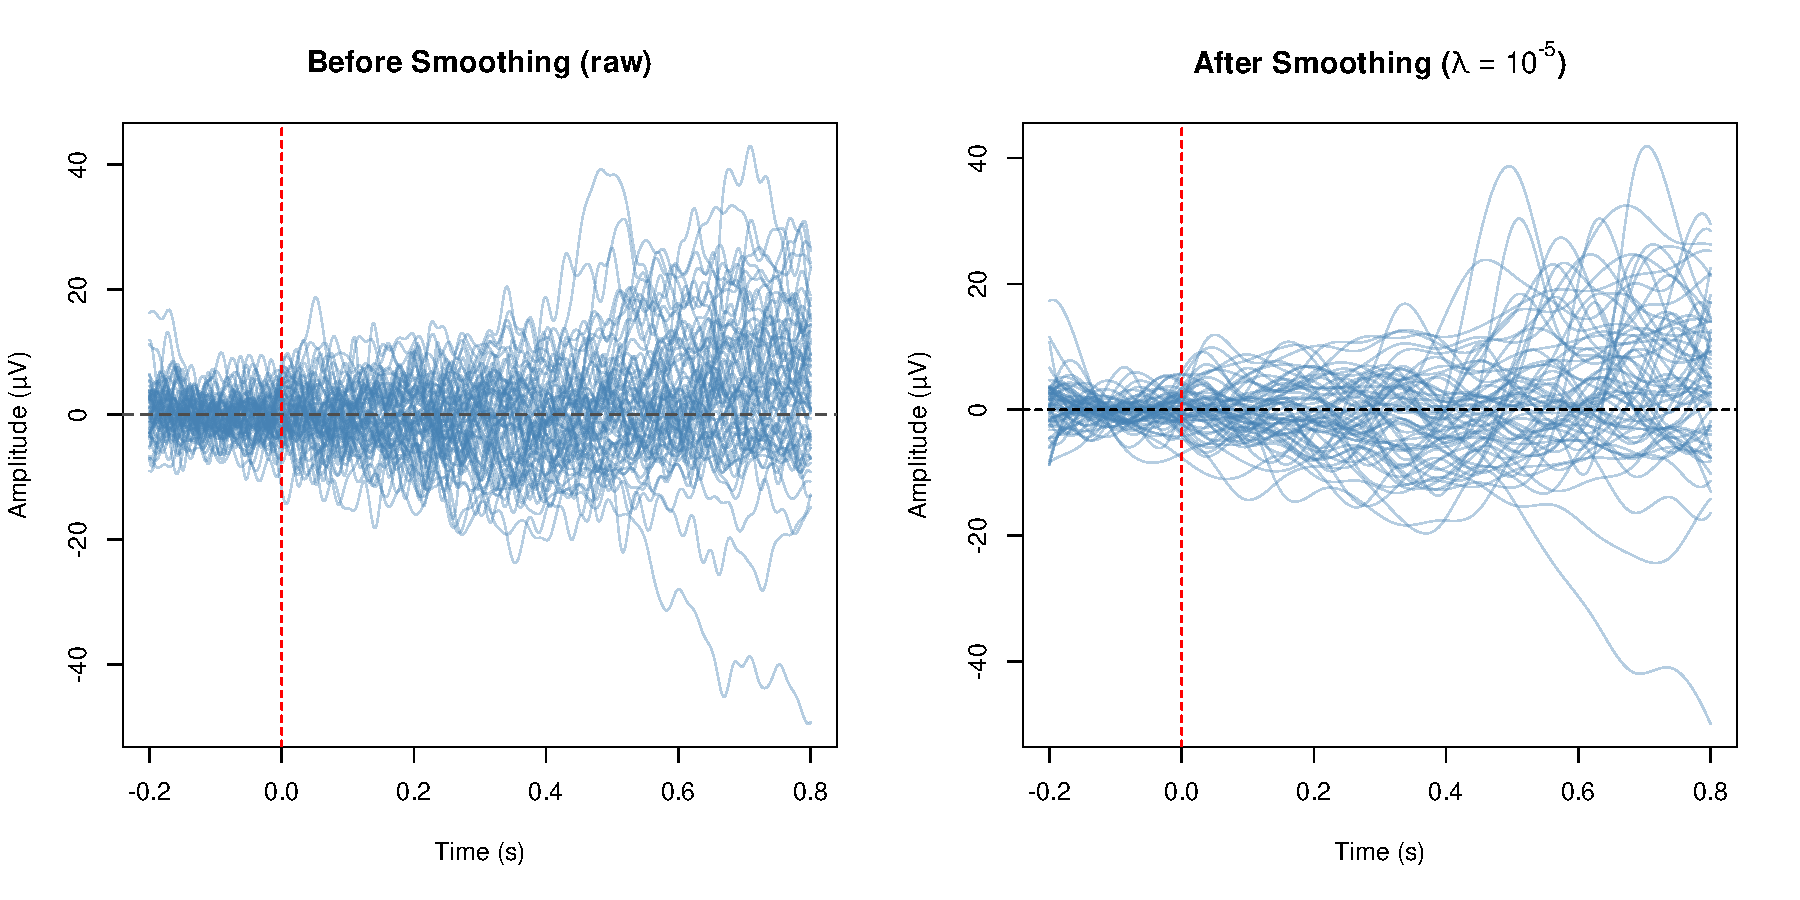
\includegraphics[width=1\textwidth]{02_before_after_smoothing.pdf}
\end{frame}

\begin{frame}{EDA}
  \begin{columns}
    \begin{column}{0.5\textwidth}
      \centering
      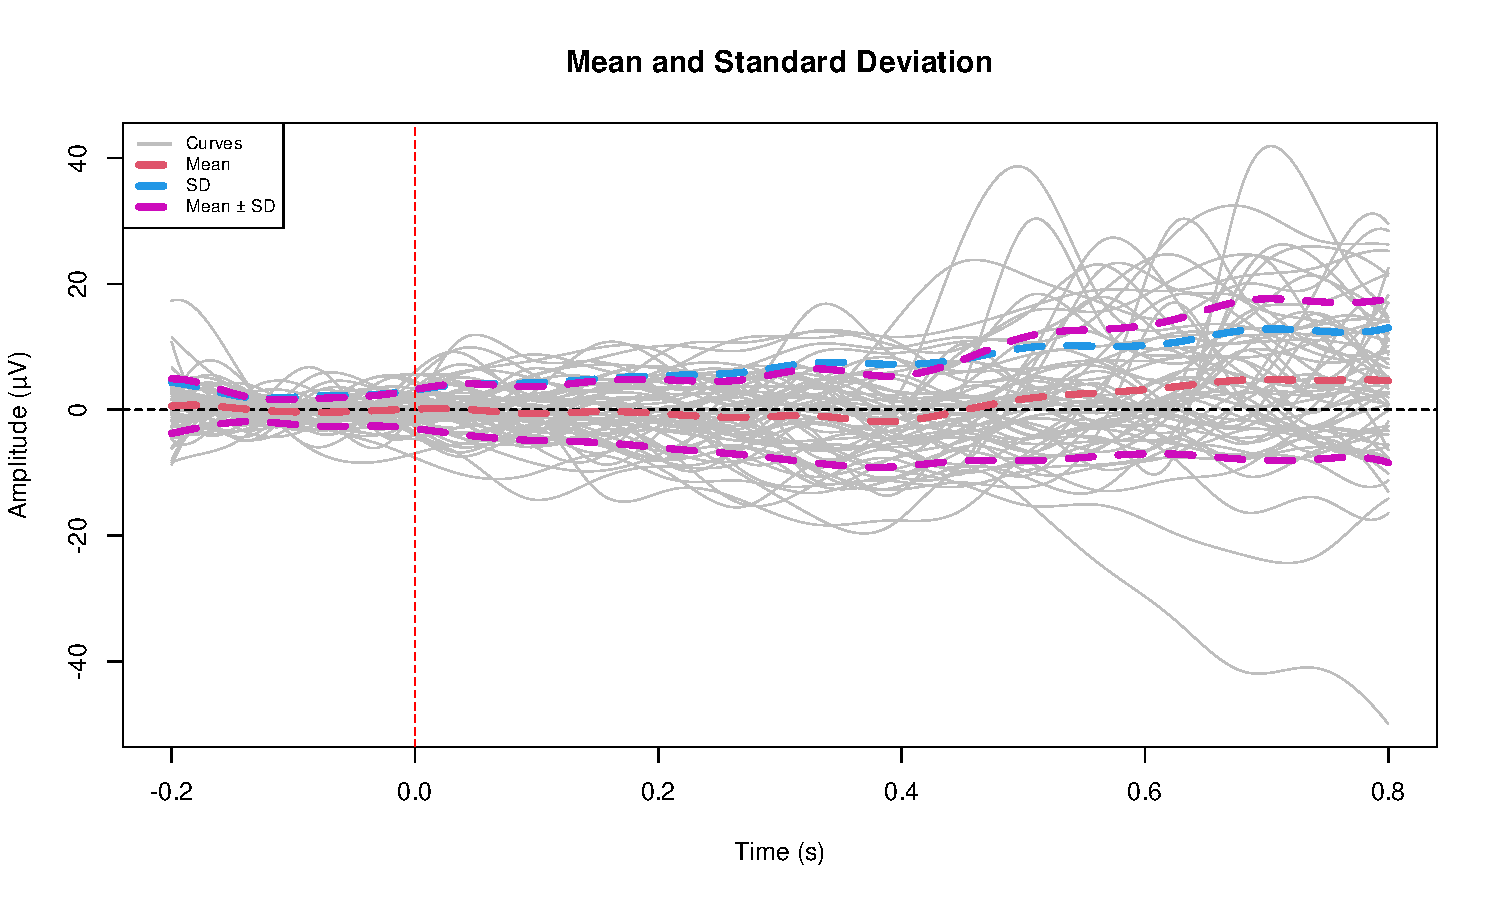
\includegraphics[width=\textwidth]{04_mean_sd.pdf}
    \end{column}
    \begin{column}{0.5\textwidth}
      \centering
      
\includegraphics[width=\textwidth]{07_covariance_image.pdf}
    \end{column}
  \end{columns}
\end{frame}

\begin{frame}{EDA}
  \begin{columns}
    \begin{column}{0.5\textwidth}
      \centering
      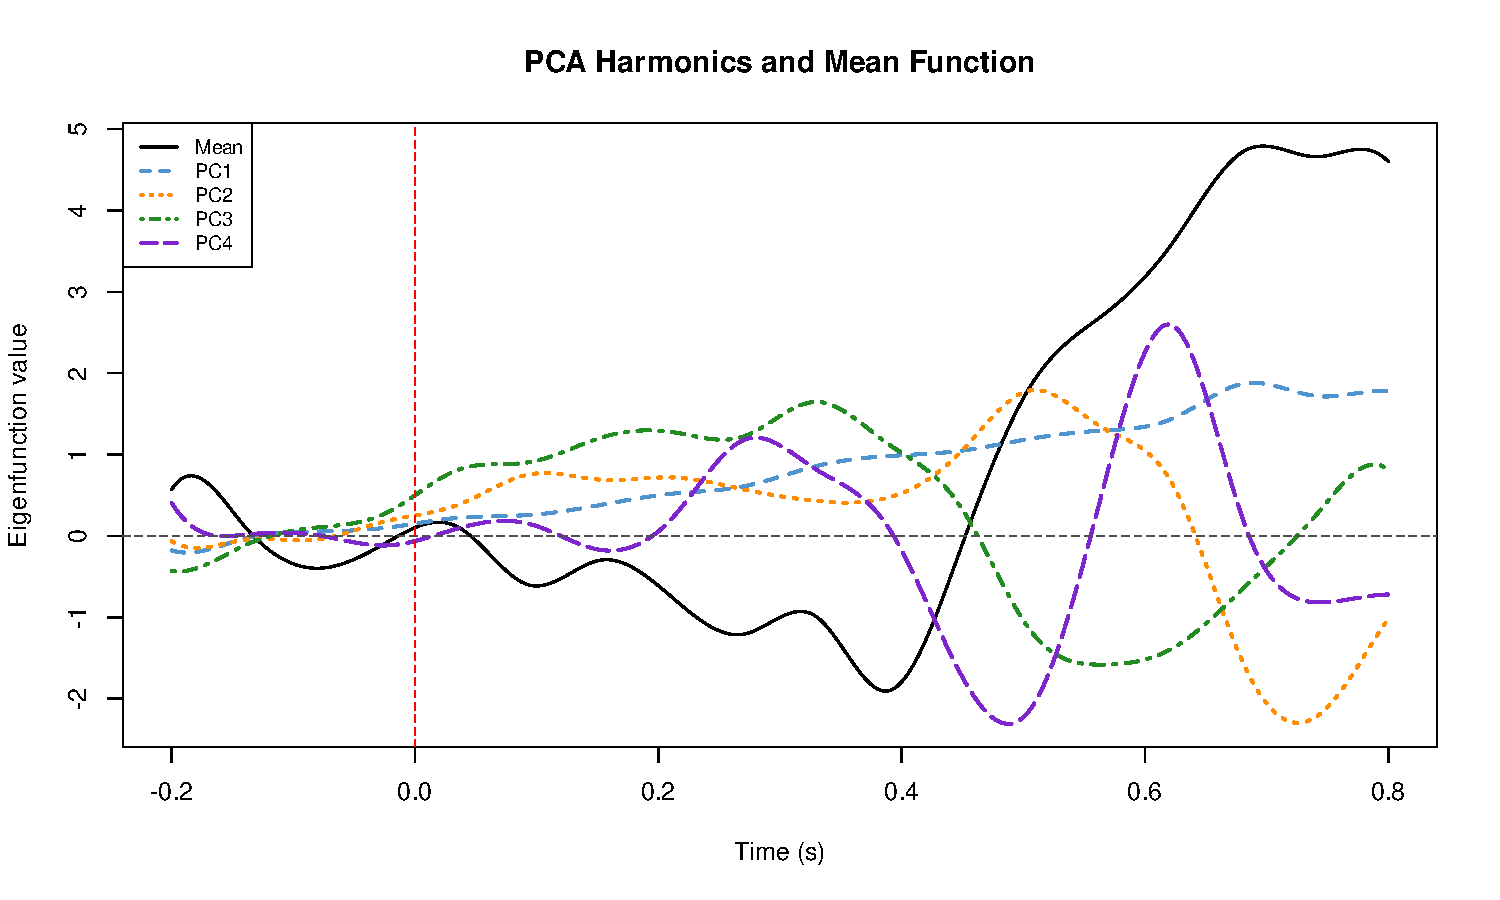
\includegraphics[width=\textwidth]{13_pca_harmonics.pdf}
      \vspace{0.2em}
      {\tiny PC1: 61.1\% \quad PC2: 13.6\% \quad PC3: 11.9\% \quad PC4: 3.3\%}
    \end{column}
    \begin{column}{0.5\textwidth}
      \centering
      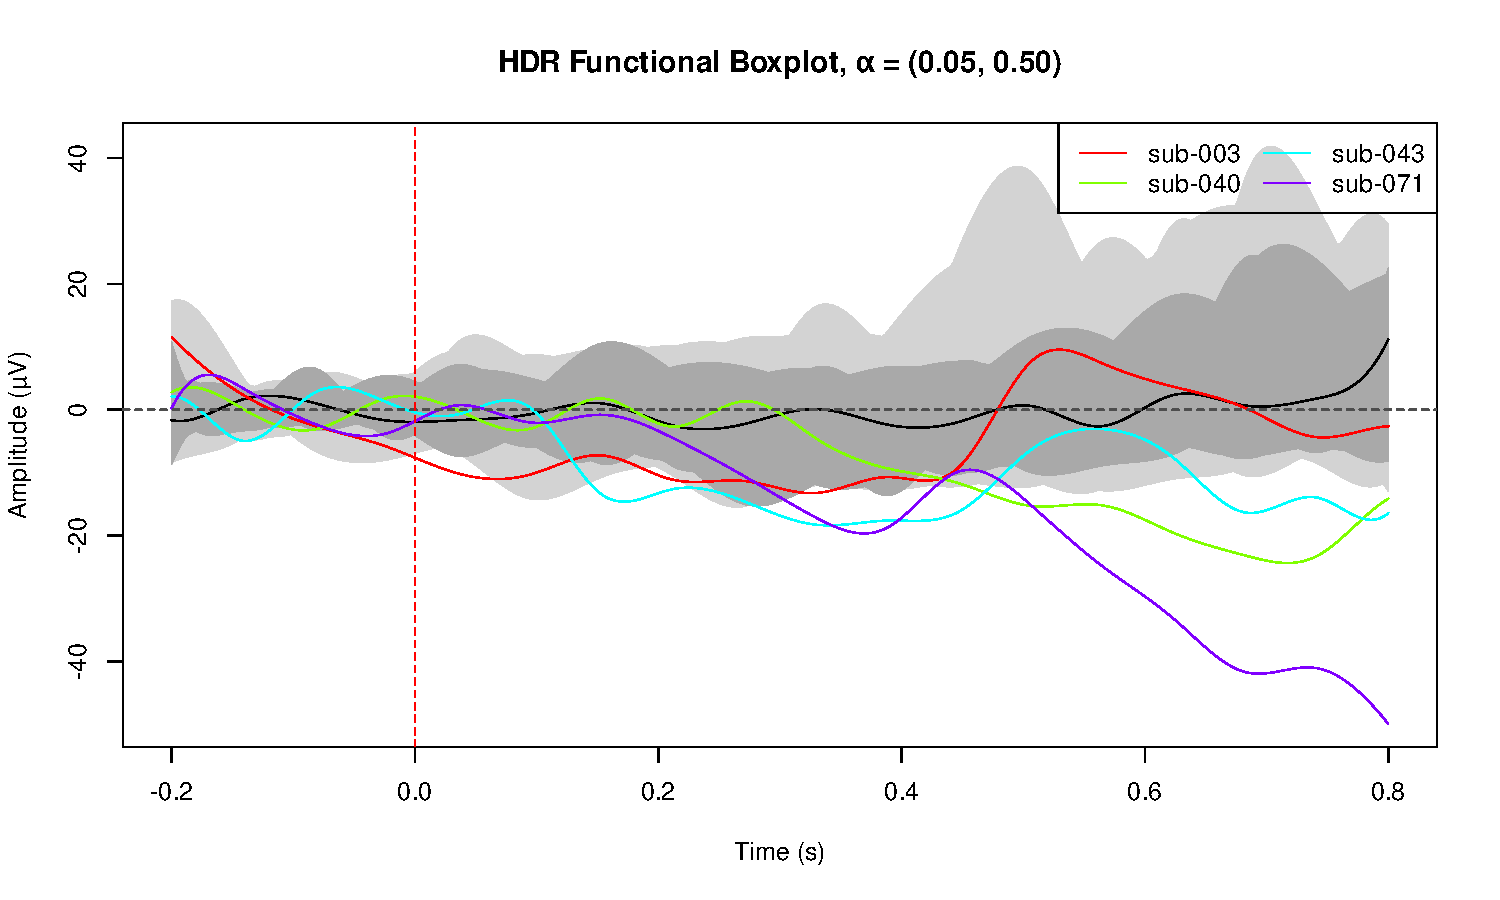
\includegraphics[width=\textwidth]{32_hdr_functional_005.pdf}
    \end{column}
  \end{columns}
  \vspace{0.5em}
  \small Magnitude outliers identified: \texttt{sub-003}, \texttt{sub-040},
  \texttt{sub-043}, \texttt{sub-071} — retained in subsequent analyses.
\end{frame}

\begin{frame}{Hypothesis Testing — Summary}
  \begin{align*}
    H_0 &: \mu_A(t) = \mu_B(t), \quad \forall\, t \in [-0.2,\, 0.8] \\
    H_1 &: \mu_A(t) \neq \mu_B(t), \quad \text{for some } t
  \end{align*}
  \begin{table}[h]
    \centering
    \small
    \begin{tabular}{l l c}
      \hline
      \textbf{Comparison} & \textbf{Test} & \textbf{p-value} \\
      \hline
      \multirow{3}{*}{ADHD vs non-ADHD}
        & L2-norm (bootstrap) & 0.7260 \\
        & F-type (bootstrap)  & 0.7140 \\
        & Permutation         & 0.5250 \\
      \hline
      \multirow{3}{*}{Female vs Male}
        & L2-norm (bootstrap) & 0.2600 \\
        & F-type (bootstrap)  & 0.2680 \\
        & Permutation         & 0.1050 \\
      \hline
      SES (Low/Mid/High) & Functional ANOVA & 0.4020 \\
      \hline
    \end{tabular}
  \end{table}
  \vspace{0.3em}
  \textbf{Conclusion:} All three hypotheses fail to reject $H_0$ at
  $\alpha = 0.05$ — no significant differences found between groups.
\end{frame}

% --- Regression Model Results ------------------------------------------------
\section{Regression Model Results}

\begin{frame}{Regression Model}
  To further investigate the relationship between EEG response curves and
  subject characteristics, a function-on-scalar regression model was fitted.
  The regression was performed on the 51 subjects with known ADHD
  classification, excluding the 11 subjects with missing ADHD status.
  The model is defined as:
  \begin{equation}
    Y_i(t) = \beta_0(t) + \beta_1(t) \cdot \text{ADHD}_i
            + \beta_2(t) \cdot \text{Female}_i + \varepsilon_i(t),
            \qquad t \in [-0.2\,\mathrm{s},\, 0.8\,\mathrm{s}]
  \end{equation}
\end{frame}

\begin{frame}{Model Summary}
  \begin{table}[ht]
    \centering
    \begin{tabular}{lrrrr}
      \toprule
      \multicolumn{5}{l}{\textbf{Constant coefficients:}} \\
      & \textbf{Estimate} & \textbf{Std. Error}
      & \textbf{t value}  & \textbf{Pr($>|t|$)} \\
      \midrule
      (Intercept) & $-0.7201$ & $1.0344$ & $-0.696$ & $0.486$ \\
      \midrule
      \multicolumn{5}{l}{\textbf{Smooth terms \& functional coefficients:}} \\
      & \textbf{edf} & \textbf{Ref.df} & \textbf{F} & \textbf{p-value} \\
      \midrule
      Intercept(\texttt{yindex}) & $10.686$ & $19.000$ & $9.299$ & $0.0237$~* \\
      ADHD(\texttt{yindex})      & $2.001$  & $2.378$  & $0.251$ & $0.8421$   \\
      Female(\texttt{yindex})    & $4.498$  & $4.794$  & $2.762$ & $0.0159$~* \\
      \midrule
      \multicolumn{5}{l}{Signif. codes:
        0 \texttt{`***'}\;
        0.001 \texttt{`**'}\;
        0.01 \texttt{`*'}\;
        0.05 \texttt{`.'}\;
        0.1 \texttt{` '}\;
        1} \\
      \midrule
      \multicolumn{3}{l}{$R^2_{\text{adj}} = 0.108$}
      & \multicolumn{2}{r}{Deviance explained $= 11.1\%$} \\
      \bottomrule
    \end{tabular}
    \caption{Summary of the regression model.}
    \label{tab:model_summary}
  \end{table}
\end{frame}

\begin{frame}{Estimated Functional Regression Coefficients}
  \centering
  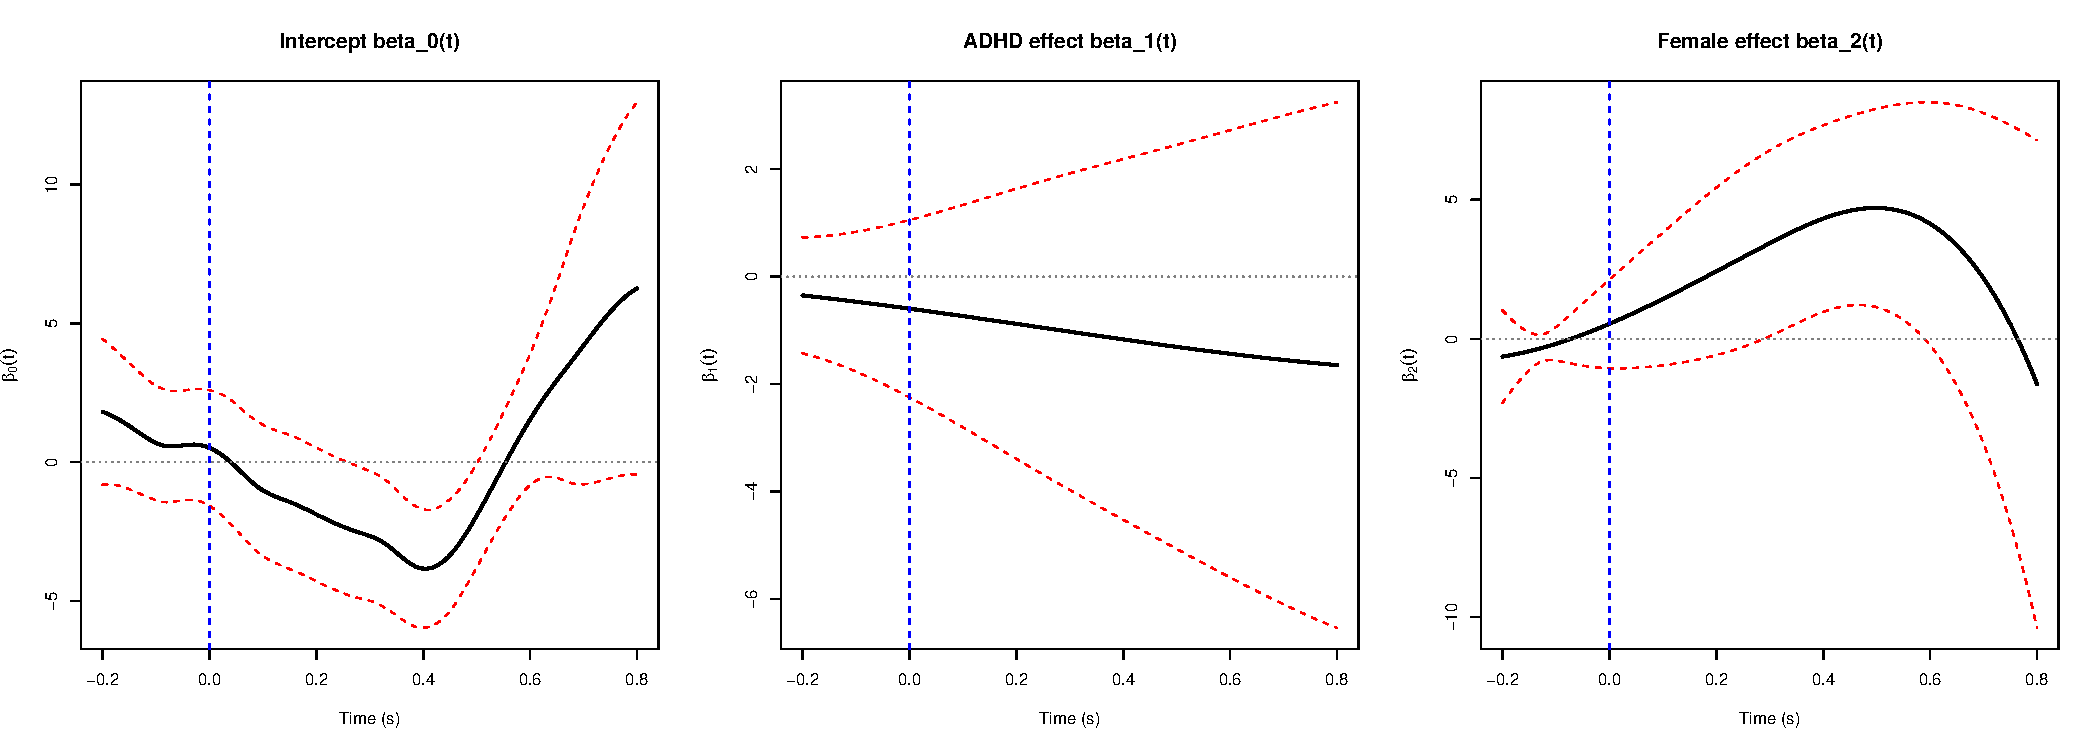
\includegraphics[width=1\textwidth]{REG_02_individual_coefficients.pdf}
\end{frame}

\begin{frame}{Observed and Fitted EEG Response Curves}
  \centering
  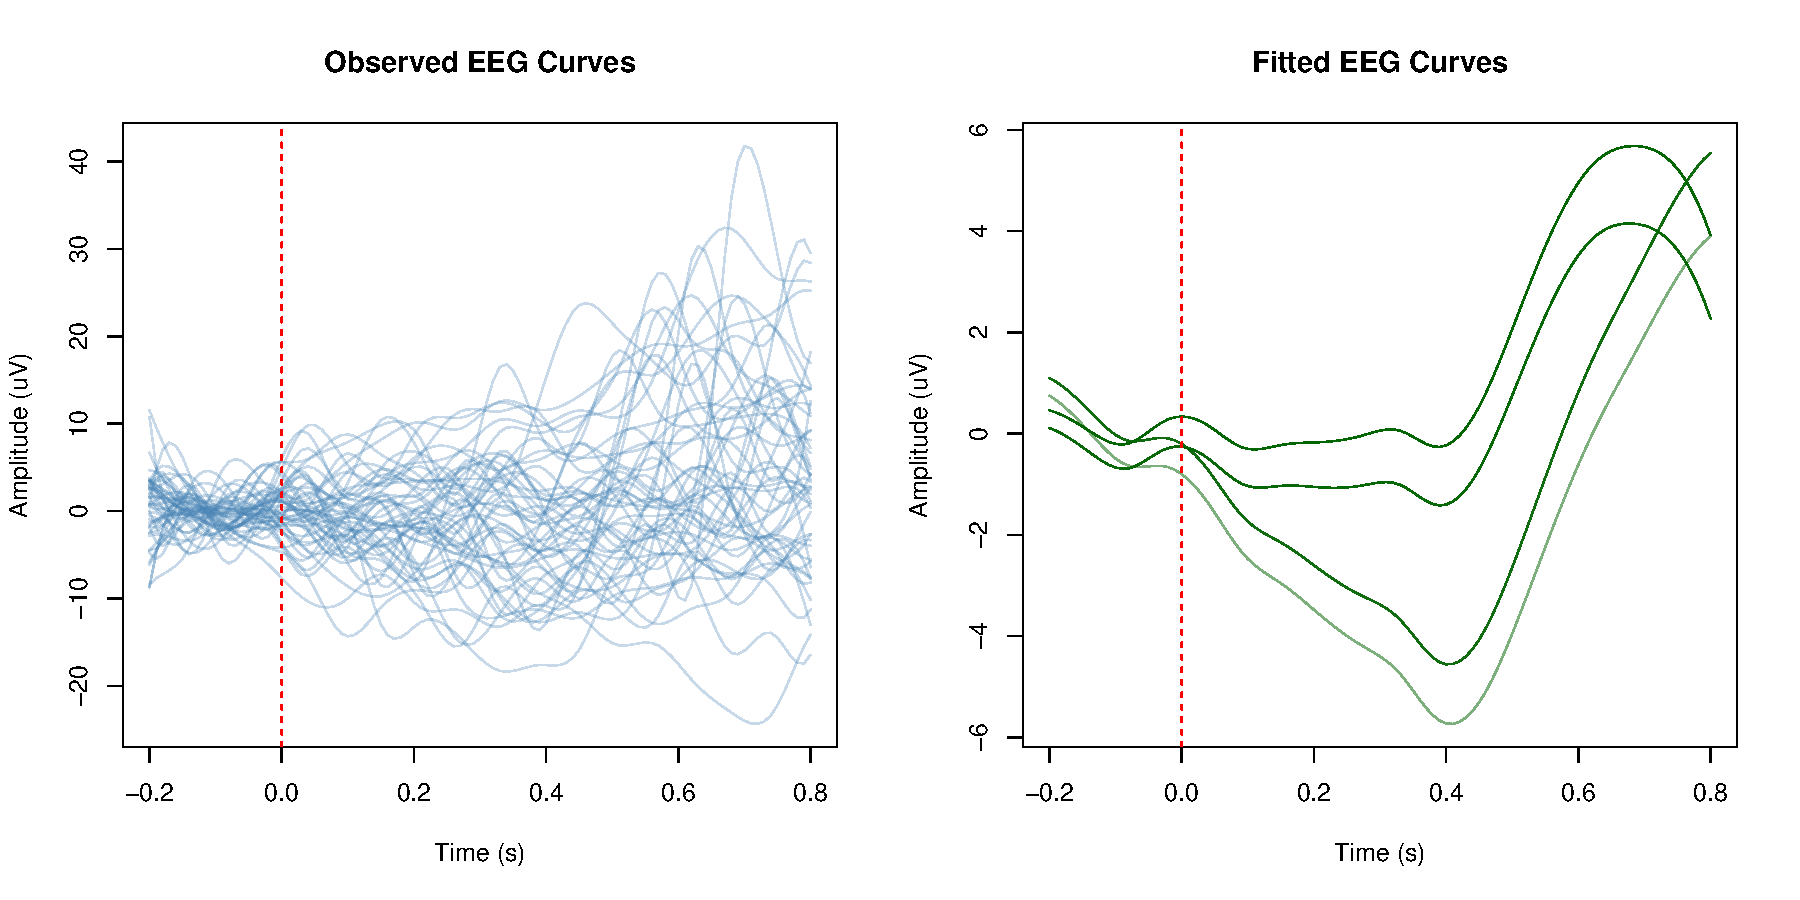
\includegraphics[width=1\textwidth]{REG_03_fitted_vs_observed.pdf}
\end{frame}

% --- Conclusions -------------------------------------------------------------
\section{Conclusions}

\begin{frame}{Conclusions}
  \begin{itemize}
    \item \textbf{Between-subject variability} is concentrated in the
      post-stimulus window ($0.4$--$0.8\,\mathrm{s}$), with the first three
      functional principal components explaining $86.6\%$ of total variance.
    \item \textbf{Function-on-scalar regression} extended the hypothesis
      testing by simultaneously modeling ADHD and gender effects on the
      EEG curves at channel FC1.
    \item \textbf{Gender} showed a statistically significant effect
      ($p = 0.016$), with female subjects exhibiting lower amplitudes in the
      post-stimulus window (0.3--0.6 s), while \textbf{ADHD} status had no
      significant effect ($p = 0.842$).
    \item The model's low explanatory power ($R^2 \approx 0.11$) indicates
      that substantial individual variability remains unexplained, suggesting
      other covariates may contribute to EEG response patterns.
  \end{itemize}
\end{frame}

% --- Acknowledgements --------------------------------------------------------
\section*{Acknowledgements}

\begin{frame}
  \textcolor{myNewColorA}{\Huge{\centerline{Thank you for your time!}}}
\end{frame}

% =============================================================================
\end{document}
